\documentclass{standalone}
\usepackage{tikz}
\usepackage{pgfplots}
\pgfplotsset{width=32cm,height=18cm,compat=1.3}
\pgfplotsset{every tick label/.append style={font=\Huge}}
\usepackage{filecontents}
\usepgfplotslibrary{fillbetween}

\usetikzlibrary{patterns}

\definecolor{citrine}{rgb}{0.89, 0.82, 0.04}
\definecolor{arylideyellow}{rgb}{0.91, 0.84, 0.42}
\definecolor{bronze}{rgb}{0.8, 0.5, 0.2}

\begin{document}
	\centering
		\vspace{1.5em}
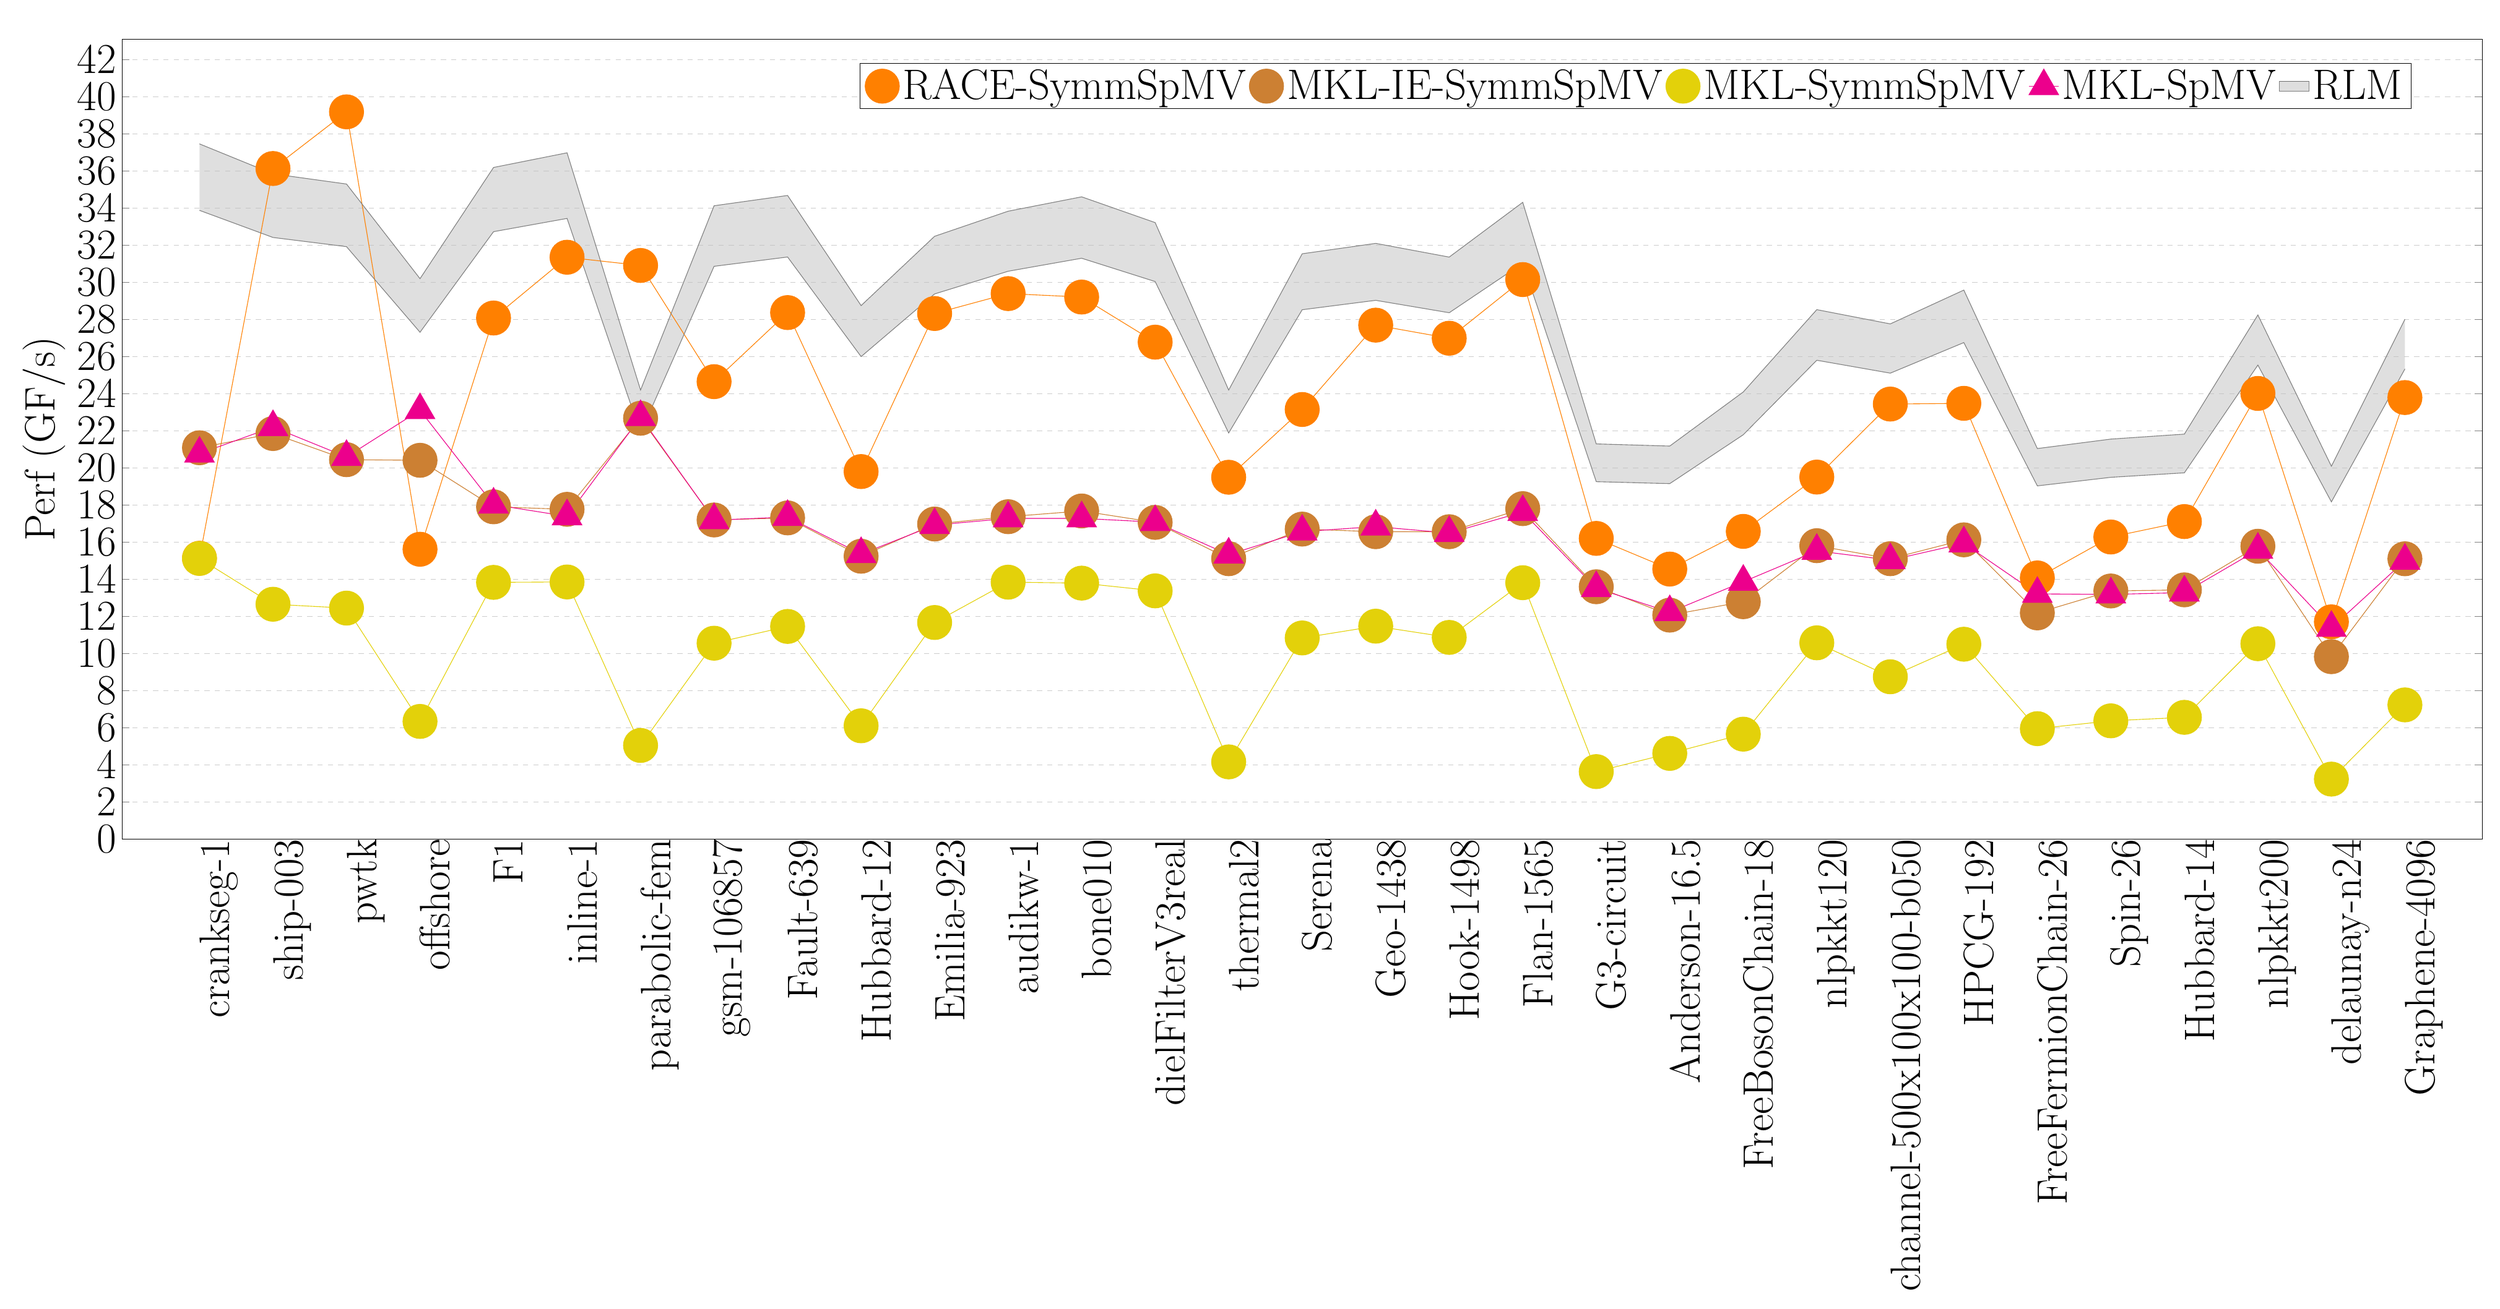
\begin{tikzpicture}
		%	\node at (13.25,15) {\LARGE{}};
			\begin{axis}[
		%	xmin=0.25, xmax=7.25,
			ymin=0, %ymax=3.25,
			xtick={1, 2, 3, 4, 5, 6, 7, 8, 9, 10, 11, 12, 13, 14, 15, 16, 17, 18, 19, 20, 21, 22, 23, 24, 25, 26, 27, 28, 29, 30, 31},
		%	ytick={0,0.5,1,1.5,2,2.5,3},
			xticklabels={crankseg-1, ship-003, pwtk, offshore, F1, inline-1, parabolic-fem, gsm-106857, Fault-639, Hubbard-12, Emilia-923, audikw-1, bone010, dielFilterV3real, thermal2, Serena, Geo-1438, Hook-1498, Flan-1565, G3-circuit, Anderson-16.5, FreeBosonChain-18, nlpkkt120, channel-500x100x100-b050, HPCG-192, FreeFermionChain-26, Spin-26, Hubbard-14, nlpkkt200, delaunay-n24, Graphene-4096},
			width  = 50cm,
			height = 18cm,
			major x tick style = transparent,
			%	minor ytick={1, 5, 10, 15, 20, 25, 30 ,35,40},
			grid = minor,	
			%add_bar_commands
			ymajorgrids = true,
			grid style={dashed, gray!40},
			ylabel = {\Huge{Perf (GF/s)}},
		%	symbolic x coords={Graphene-2048-2048, Graphene-4096-4096, Spin-24-24-24},
			x tick label style={rotate=90, anchor=north east, inner sep=0mm, font={\Huge}},
			tick label style={font={\Huge}},
			scaled y ticks = false,
			enlarge x limits=0.035,
			legend cell align=left,
			legend style={font=\Huge},
			legend columns=-1,
			legend style={
				%at={(1,1.05)},
				%anchor=south east,
				%column sep=1ex,
				legend pos=north east
			},
			%spl_legend_code
			title= {\Huge\scalebox{1.5}{{}}}
			]

\addplot[name path=1, mark=*, mark size=10pt, mark options={orange}, draw=orange ] plot coordinates{(1,15.130207) (2,36.140175) (3,39.194893) (4,15.613967) (5,28.080251) (6,31.356939) (7,30.913152) (8,24.649314) (9,28.372987) (10,19.802304) (11,28.323231) (12,29.396679) (13,29.210280) (14,26.778583) (15,19.496395) (16,23.148677) (17,27.696097) (18,26.990050) (19,30.152423) (20,16.199662) (21,14.545610) (22,16.577436) (23,19.505411) (24,23.441453) (25,23.480804) (26,14.069287) (27,16.275497) (28,17.107030) (29,24.014713) (30,11.700657) (31,23.793009)};
\addplot[name path=2, mark=*, mark size=10pt, mark options={bronze}, draw=bronze ] plot coordinates{(1,21.085770) (2,21.852290) (3,20.443853) (4,20.410004) (5,17.902724) (6,17.767401) (7,22.676625) (8,17.193174) (9,17.304731) (10,15.238413) (11,16.975884) (12,17.369550) (13,17.678201) (14,17.062434) (15,15.104626) (16,16.700991) (17,16.560236) (18,16.560155) (19,17.804302) (20,13.593018) (21,12.063563) (22,12.785401) (23,15.806911) (24,15.105072) (25,16.121380) (26,12.183172) (27,13.365014) (28,13.425972) (29,15.776211) (30,9.822844) (31,15.101306)};
\addplot[name path=3, mark=*, mark size=10pt, mark options={citrine}, draw=citrine ] plot coordinates{(1,15.119512) (2,12.650132) (3,12.441833) (4,6.333084) (5,13.829457) (6,13.851336) (7,5.038517) (8,10.549724) (9,11.453661) (10,6.097175) (11,11.666272) (12,13.840258) (13,13.788486) (14,13.371284) (15,4.151923) (16,10.832944) (17,11.467940) (18,10.862180) (19,13.810900) (20,3.627569) (21,4.609543) (22,5.646701) (23,10.570603) (24,8.739723) (25,10.494392) (26,5.942178) (27,6.364800) (28,6.553474) (29,10.521455) (30,3.223295) (31,7.224236)};
\addplot[name path=4, mark=triangle*, mark size=10pt, mark options={magenta}, draw=magenta ] plot coordinates{(1,20.769206) (2,22.199856) (3,20.590162) (4,23.111813) (5,18.019958) (6,17.389334) (7,22.738380) (8,17.180456) (9,17.354518) (10,15.352748) (11,16.918081) (12,17.275771) (13,17.277571) (14,17.077006) (15,15.326098) (16,16.566454) (17,16.836613) (18,16.487552) (19,17.619697) (20,13.517244) (21,12.222770) (22,13.860350) (23,15.527179) (24,15.026985) (25,15.929758) (26,13.208086) (27,13.177933) (28,13.278095) (29,15.587776) (30,11.374282) (31,14.997639)};
\addplot[name path=5, mark=nomarks, mark size=10pt, mark options={gray}, draw=gray ] plot coordinates{(1,33.88391443321596) (2,32.422674442241515) (3,31.927255075719515) (4,27.31242686610072) (5,32.73450624945676) (6,33.448600498754566) (7,21.882932745899687) (8,30.867359296056815) (9,31.369144841935526) (10,25.99949761373668) (11,29.379078942831114) (12,30.601322242191323) (13,31.302577971608205) (14,30.046007594627486) (15,21.88158503049584) (16,28.526731688642375) (17,29.03360063990211) (18,28.36529966442702) (19,31.034442066523432) (20,19.257114640970986) (21,19.15212087640105) (22,21.788631100011006) (23,25.802699411960024) (24,25.107708815137492) (25,26.75615029292358) (26,19.030557606095222) (27,19.49194495374786) (28,19.734157095876782) (29,25.54372630375391) (30,18.167625421267388) (31,25.33332832179717)};
\addplot[name path=6, mark=nomarks, mark size=10pt, mark options={gray}, draw=gray ] plot coordinates{(1,37.46778999826765) (2,35.8519957774786) (3,35.30417628565139) (4,30.201241246169065) (5,36.196809795072376) (6,36.98643324381514) (7,24.197473709408307) (8,34.13217614467821) (9,34.68703516175563) (10,28.74944447672806) (11,32.486481523322865) (12,33.83800055626925) (13,34.61342756475907) (14,33.2239507055977) (15,24.195983447182904) (16,31.543982155710317) (17,32.10446224604561) (18,31.365475590472187) (19,34.31693113125188) (20,21.293924843381376) (21,21.177825969097313) (22,24.09319785097371) (23,28.53183108053272) (24,27.763331862892418) (25,29.586127727752036) (26,21.04340504520145) (27,21.553592977701964) (28,21.821423711786828) (29,28.245466585881726) (30,20.08920118697836) (31,28.012814971218024)};
\addplot[fill=lightgray,opacity=0.5]
fill between[of= 5 and 6];
	%addplot cmd

	\legend{RACE-SymmSpMV, MKL-IE-SymmSpMV, MKL-SymmSpMV, MKL-SpMV, , ,RLM}

	\end{axis}			
\end{tikzpicture}

\end{document}

